\chapter{Pendahuluan}
\section{Latar Belakang}

Terumbu karang adalah ekosistem bawah laut yang terbentuk dari sekumpulan karang. Selain berfungsi sebagai ekosistem di bawah laut, terumbu karang juga berfungsi sebagai pemecah gelombang. Sebagian besar kepulauan di wilayah pasific di kelilingi oleh terumbu karang yang tumbuh di laut dangkal yang dekat dengan pantai \cite{DemirbilekBoussinesq}.

\begin{figure}[htp]
    \begin{center}
        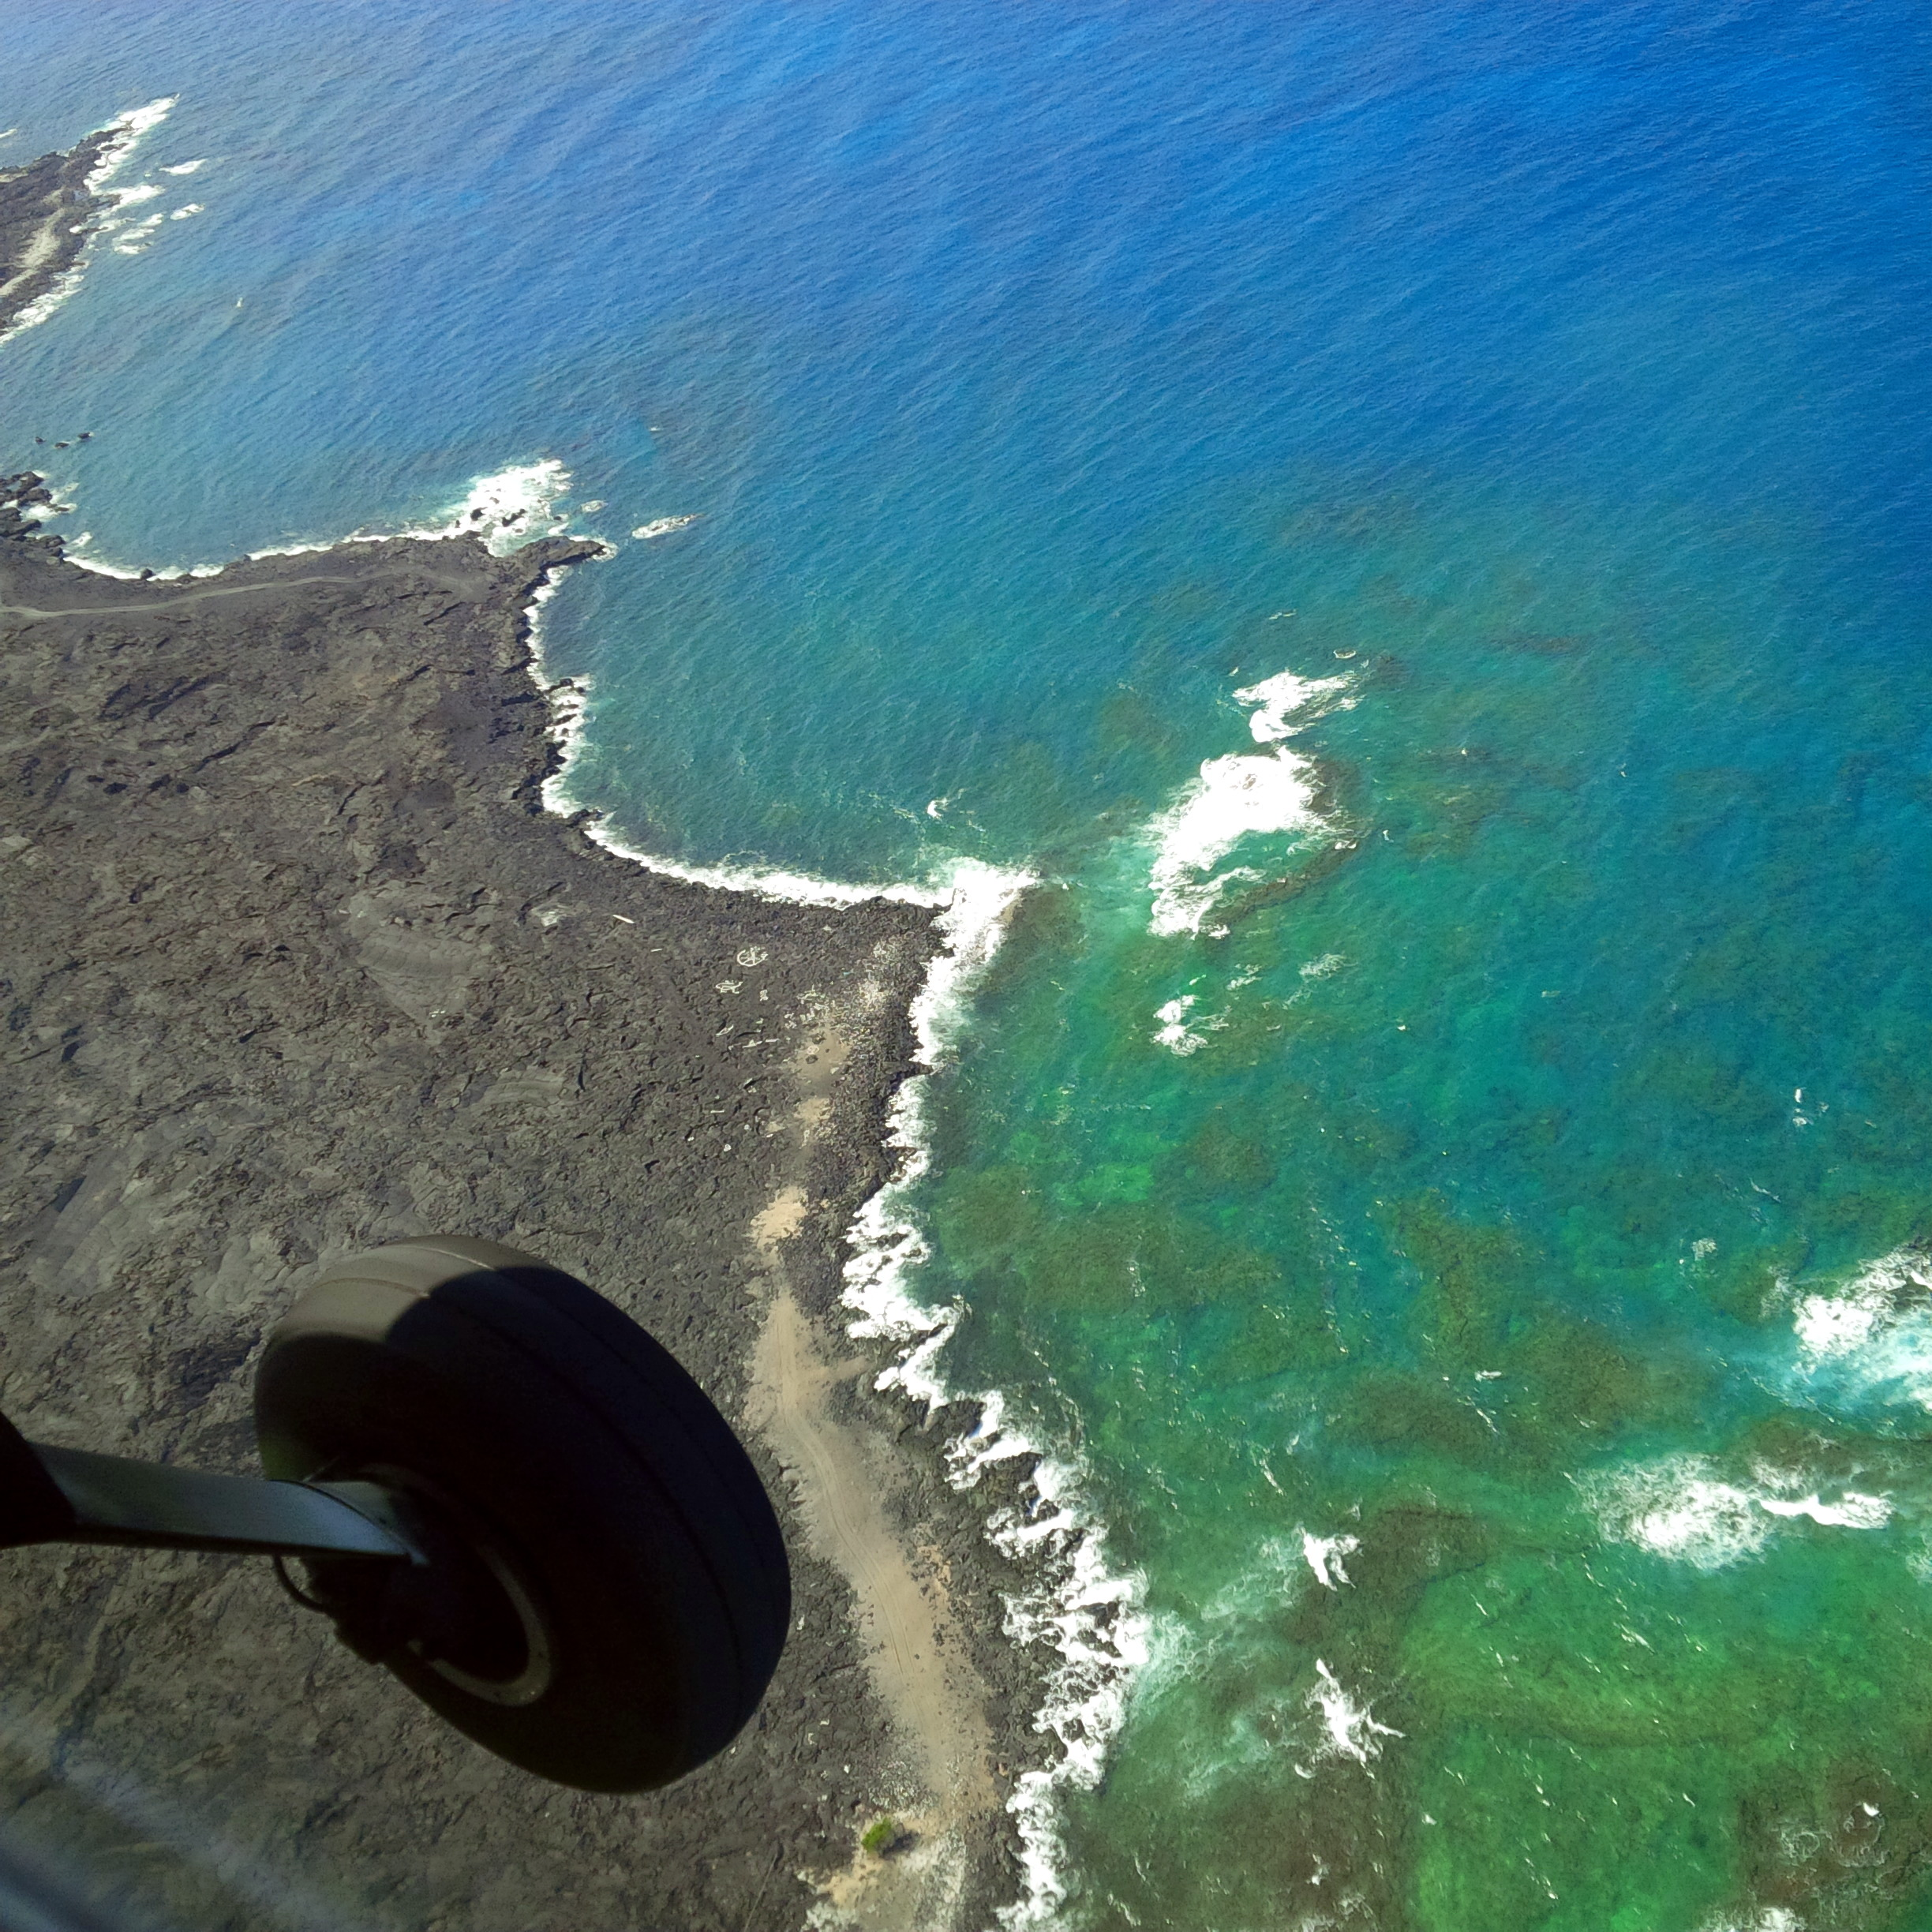
\includegraphics[scale=0.1]{./images/hawai_coral.jpg}
    \end{center}
    \caption{Terumbu Karang di tepi pantai di sekitar Hawai.}
\end{figure}

Gelombang yang melewati terumbu karang akan teredam kecepatannya \cite{DemirbilekReport}. Hal ini akan mempengaruhi naiknya gelombang ke daratan di atas batas normal, atau dalam literatur lain disebut \emph{runup} gelombang \cite{nielsen1991wave}. Teredamnya kecepatan gelombang disebabkan oleh bertumbukannya dasar gelombang dengan karang. Dalam beberapa kasus, hal ini menyebabkan pecahnya gelombang \cite{DemirbilekReport}

Namun efektifitas dari terumbu karang dalam meredam gelombang masih menjadi perdebatan para peneliti. Yang selama ini dilakukan dalam mempelajari redaman dari terumbu karang adalah eksperimen di laboratorium. Seperti yang dilakukan Yau et al (2012)\cite{YAO201230}, dia mengerjakannya dengan menggunakan model \emph{Boussinesq} 1 dimensi untuk memodelkan transformasi gelombang saat melewati terumbu karang.  Namun cara mempelajari ini tergolong mahal dan membutuhkan pemodelan matematika yang dalam untuk memodelkan pecahnya gelombang.

Selama ini metode yang ada untuk memprediksi tinggi gelombang \emph{runup} pada terumbu karang masih tergolong baru. Metodenya sendiri terbagi menjadi 2. Metode yang pertama dilakukan dengan pendekatan klasik, dan di lakukan secara analitis. Yakni dengan melakukan eksperimen dan observasi, lalu di cari model matematika yang tepat. Model yang demikian sulit untuk dikembangkan dan beradaptasi dengan kondisi lingkungan yang berbeda. Prediksi yang didapat dari model yang demikian pun masih belum sempurna \cite{DemirbilekBoussinesq}. Sedangkan metode yang kedua dilakukan dengan pendekatan \emph{soft computing}.

Pada TA ini kami menggunakan Pembelajaran Mesin untuk memprediksi \emph{runup} gelombang. Metode yang digunakan disini adalah \emph{supervised learning}, dengan menggunakan data dari Demirbilek et al (2007)\cite{DemirbilekReport}. Dari data hasil \emph{training} dan \emph{testing} dengan konfigurasi neural network. Diharapakan mendapatkan model dengan akurasi yang tinggi. Sehingga efisiensi dari terumbu karang dalam memecahkan gelombang dapat dipelajari dengan baik.

\section{Perumusan Masalah}
Rumusan masalah yang ingin yang angkat pada TA ini adalah
\begin{enumerate}
    \item Bagaimana melakukan pemodelan supervised learning dengan data eksperimen yang dilakukan di laboratorium?
    \item Bagaimana akurasi dari model prediksi runup gelombang yang telah dibuat?
    \item Seberapa efisien terumbu karang dalam meredam gelombang?
\end{enumerate}
\section{Tujuan}
Berikut adalah tujuan yang ingin dicapai pada penulisan proposal/TA.
\begin{enumerate}
    \item Memodelkan data hasil eksperimen di laboratorium menggunakan \emph{supervised learning}
    \item Mengetahui akurasi Artificial Neural Network untuk prediksi \emph{runup} gelombang pada terumbu karang.
    \item Mengetahui efisiensi dari terumbu karang dalam meredam gelombang.
\end{enumerate}
\section{Batasan Masalah}
Untuk memastikan hasil yang cukup akurat. Lingkupan masalah diperkecil menjadi:
\begin{enumerate}
    \item Data berasal dari eksperimen pada laboratorium dinamika oleh Demerbilek (2007).
    \item Metode yang digunakan pada eksperimen ini adalah Artificial Neural Network.
\end{enumerate}
\section{Rencana Kegiatan}
Rencana kegiatan yang akan saya lakukan adalah sebagai berikut:
\begin{itemize}
    \item Studi literatur: Pengumpulan informasi dan referensi.
    \item Penentuan Topik
    \item Analisis dan Perancangan Sistem
    \item Implementasi Sistem
    \item Analisa Hasil Implementasi
    \item Penulisan Laporan
\end{itemize}
\section{Jadwal Kegiatan}

Laporan proposal ini akan dijadwalkan sesuai dengan tabel berikut:

 
\begin{table}[h!]
  \centering
    \caption{Jadwal kegiatan proposal tugas akhir}
  \label{Novella}
  \begin{tabular}{|c|m{2.5cm}|m{0.01cm}|m{0.01cm}|m{0.01cm}|m{0.01cm}|m{0.01cm}|m{0.01cm}|m{0.01cm}|m{0.01cm}|m{0.01cm}|m{0.01cm}|m{0.01cm}|m{0.01cm}|m{0.01cm}|m{0.01cm}|m{0.01cm}|m{0.01cm}|m{0.01cm}|m{0.01cm}|m{0.01cm}|m{0.01cm}|m{0.01cm}|m{0.01cm}|m{0.01cm}|m{0.01cm}|}
    \hline
    \multirow{2}{*}{\textbf{No}} & \multirow{2}{*}{\textbf{Kegiatan}} & \multicolumn{24}{|c|}{\textbf{Bulan ke-}} \\
    \hhline{~~------------------------}
    {} & {} & \multicolumn{4}{|c|}{\textbf{1}} & \multicolumn{4}{|c|}{\textbf{2}} & \multicolumn{4}{|c|}{\textbf{3}} & \multicolumn{4}{|c|}{\textbf{4}} & \multicolumn{4}{|c|}{\textbf{5}} & \multicolumn{4}{|c|}{\textbf{6}}\\
    \hline
    1 & Studi Literatur & \cellcolor{blue!25} & \cellcolor{blue!25} & \cellcolor{blue!25} & \cellcolor{blue!25}& \cellcolor{blue!25} & \cellcolor{blue!25} & \cellcolor{blue!25} & \cellcolor{blue!25}& \cellcolor{blue!25} & \cellcolor{blue!25} & \cellcolor{blue!25} & \cellcolor{blue!25}& \cellcolor{blue!25} & \cellcolor{blue!25} & \cellcolor{blue!25} & \cellcolor{blue!25}& \cellcolor{blue!25} & \cellcolor{blue!25} & \cellcolor{blue!25} & \cellcolor{blue!25}& \cellcolor{blue!25} & \cellcolor{blue!25} & \cellcolor{blue!25} & \cellcolor{blue!25}\\
    \hline
    2 & Analisis dan Perancangan Sistem &  {} & {} & {} & {}  & \cellcolor{blue!25} & \cellcolor{blue!25} & \cellcolor{blue!25} & \cellcolor{blue!25} & \cellcolor{blue!25} & \cellcolor{blue!25} & \cellcolor{blue!25} & \cellcolor{blue!25} & {} & {} & {} & {}& {} & {} & {} & {}& {} & {} & {} & {}\\
    \hline
    3 & Implementasi Sistem &  {} & {} & {} & {} & {} & {} & {} & {}& \cellcolor{blue!25} & \cellcolor{blue!25} & \cellcolor{blue!25} & \cellcolor{blue!25} & \cellcolor{blue!25} & \cellcolor{blue!25} & \cellcolor{blue!25} & \cellcolor{blue!25} & {} & {} & {} & {}& {} & {} & {} & {}\\
    \hline
    4 & Analisa Hasil Implementasi &  {} & {} & {} & {} & {} & {} & {} & {}& {} & {} & {} & {} & \cellcolor{blue!25} & \cellcolor{blue!25} & \cellcolor{blue!25} & \cellcolor{blue!25} & \cellcolor{blue!25} & \cellcolor{blue!25} & \cellcolor{blue!25} & \cellcolor{blue!25} & {} & {} & {} & {}\\
    \hline
    5 & Penulisan Laporan & {} & {} & {} & {} & \cellcolor{blue!25} & \cellcolor{blue!25} & \cellcolor{blue!25} & \cellcolor{blue!25}& \cellcolor{blue!25} & \cellcolor{blue!25} & \cellcolor{blue!25} & \cellcolor{blue!25}& \cellcolor{blue!25} & \cellcolor{blue!25} & \cellcolor{blue!25} & \cellcolor{blue!25}& \cellcolor{blue!25} & \cellcolor{blue!25} & \cellcolor{blue!25} & \cellcolor{blue!25}& \cellcolor{blue!25} & \cellcolor{blue!25} & \cellcolor{blue!25} & \cellcolor{blue!25}\\
    \hline
  \end{tabular}
\end{table}

